\documentclass{jfm}

% paper sizing
\usepackage[papersize={8.5in, 11.0in}]{geometry}

% enable figures
\usepackage{graphicx}

% set path to figures
\graphicspath{{figures/}}

% enable number citations
\usepackage{natbib}

% better equations
\usepackage{amsmath}

% enable links
\usepackage{hyperref}
\hypersetup{
    colorlinks=true,
    linkcolor=[rgb]{0.86, 0.20, 0.18},  % red \ref{}
    citecolor=[rgb]{0.21, 0.44, 0.72}   % blue \cite{}
}

% symbol shortcuts
%\newcommand{\del}{\boldsymbol{\nabla}}
\newcommand{\del}{\nabla}


%--------------------------------------------------
% PREAMBLE
%--------------------------------------------------
\title[Magnetorotational instability]{Magnetorotational instability: a review}

\author[S. Sim, D.~P. Larson, and W. Lee]{Shi Sim, David P. Larson, 
    and Wonjae Lee}

\affiliation{University of California, San Diego}

\begin{document}

\maketitle


%--------------------------------------------------
% ABSTRACT
%--------------------------------------------------
\begin{abstract}
We review current research on magneotorotational instability (MRI) as a 
mechanism for momentum transporation in accretion disks.
\end{abstract}


%--------------------------------------------------
% INTRO
%--------------------------------------------------
\section{Introduction}
\label{sec:intro}
Turbulence generating magnetorotational Instability (MRI) was first discovered 
by \cite{Velikhov1959} and \cite{Chandrasekhar1960} and was later re-discovered by 
\cite{Balbus1998} for astrophysical applications. MRI has since then 
been confirmed by robust numerical simulations although not experimentally or
through observations. To understand the importance of MRI, we have to look into
the accretion disk theory where many astrophysical phenomena take place in.

Accretion disks are disk made up of gas, dust, and plasma that rotates around 
and gradually collapses onto an object in the center, e.g leading to formation
of a star. However, accretion can happen only with an efficient mechanism for 
rapidly transporting angular momemtum outwards. It was suggested that 
turbulence drives angular momentum outwards but there was no known mechanism 
that would generate turbulence. These Keplerian disks satisfies the Rayleigh 
stability criterion \citep[see][]{Rayleigh1916} against centrifugal instability.
Thus, there has to be other mechanisms that generates turbulence and this is where 
MRI and non-linear hydrodynamic instablities comes into the picture. There has
been other mechanisms suggested but MRI seem like the most probable explanation
at this point.

MRI is not only applicable to astrophysical phenomena but geophysical ones as 
well, e.g. the Earth's magnetic field. It is used to better understand how planetary
magnetic field might  have formed on Earth or other planets and how and why the
field is sustained or decayed through time.

In this report, we attempt to explain and illustrate the instability in an 
astrophysical sense and go through what has been done experimentally and 
numerically in terms of MRI.



%--------------------------------------------------
% PHYSICAL EXPLANATION
%--------------------------------------------------
\section{Physical Explanation}


%
% CONDUCTING FLUID
%
\subsection{Perfectly conducting fluid in magnetic field}

The magnetic field lines are tied to the conducting fluid in which they are embedded.
We can show this by comparing a transport equation of magnetic field with a equation for a line element moving with fluid. 
We first combine Ohm's Law in ideal 
conductor and Faraday's equation to get a transport equation for magnetic 
field,
\begin{align}
    \frac{\partial \mathbf{B}}{\partial t} &= \del \times (\mathbf{u}\times \mathbf{B}) \nonumber \\
    &=\mathbf{B}\cdot\del \mathbf{u} - {\mathbf{u}\cdot\del}\mathbf{B} -\mathbf{B}\del\cdot\mathbf{u}.
\end{align}
Assuming incompressibility, we get,
\begin{align}
    \frac{D \mathbf{B}}{D t} = (\mathbf{B}\cdot \del) \mathbf{u},
\end{align}
where $\frac{D}{Dt}$ is the convective derivative $\frac{D}{Dt}=\frac{\partial}{\partial t}+(\mathbf{u}\cdot\del)$.

Considering a short line element $d\mathbf{l}$ moving with fluid, we can express 
the rate of change of $d\mathbf{l}$ as
\begin{align}
    \frac{D}{Dt}\left(d\mathbf{l}\right) = \mathbf{u}(\mathbf{x}+d\mathbf{l})-\mathbf{u}(\mathbf{x})=(d\mathbf{l}\cdot\del)\mathbf{u}.
\end{align}
Comparing two equations above, we can conclude that $\mathbf{B}$ and 
$d\mathbf{l}$ obey the same equation \cite[see][]{Davidson2001}. Therefore, the 
field lines are frozen into the fluid.


%
% MAGNETIC TENSION
%
\subsection{Magnetic tension}

When the fluid elements are displaced from their equilibrium position, the 
magnetic field lines move together with fluid elements and behave like elastic
bands frozen-into the fluid. Using Ampere's law, the Lorenz force 
$(\mathbf{J}\times\mathbf{B})$ may be written as
\begin{align}
    \mathbf{J}\times\mathbf{B} &= - \del\left(\frac{B^2}{2\mu}\right) +\frac{(\mathbf{B}\cdot \del)\mathbf{B}}{\mu}
    =- \del\left(\frac{B^2}{2\mu}\right)+\frac{\partial}{\partial s} \left[\frac{B^2}{2\mu}\right]\hat{e}_t - \frac{B^2}{\mu R}\hat{e}_n
\end{align} 
where $R$ is radius of curvature and $s$ is a coordinate along a magnetic 
field line. $\hat{e}_t$ and $\hat{e}_n$ are tangential and normal unit vectors 
respectively. The last two terms are magnetic tension forces in tangential and 
normal directions. These forces can also be interpreted as tensile stress of 
$B^2/2\mu$ acting on the end of the tube \cite[see][]{Davidson2001}. 

This tensile force which is also know as Faraday or Maxwell tension is 
analogous to a force acting on a spring. Considering a displacement 
$\boldsymbol{\xi}=\mathbf{v}\delta t$, the Faraday's equation can be written 
as $\delta \mathbf{B} = ikB\boldsymbol{\xi}$. The magnetic tension for small 
displacement per unit density $\rho$ is
\begin{align}
    \frac{(\mathbf{B}\cdot\del)\delta \mathbf{B}}{\mu \rho}=\frac{ikB\delta \mathbf{B}}{\mu \rho} = -\frac{k^2 B^2}{\mu\rho} \boldsymbol{\xi} = -K \boldsymbol{\xi},
\end{align}
where $K$ is comparable to the spring constant \cite[see][]{Wiki:MRI,Balbus1998}. The 
equation has same form of Hooke's Law for a spring.


%
% MRI
%
\subsection{Magnetoroational instability}
Consider Keplerian motion of conducting fluid orbiting around a central body of mass $M_c$.
Two adjacent fluid elements $m_i$ and $m_o$ at radial position $r_i$ and $r_o$ are orbiting around gravitational center with angular velocity $\Omega_i=\sqrt{\frac{GM_c}{r_i^{3}}}$ and $\Omega_o=\sqrt{\frac{GM_c}{r_o^{3}}}$ respectively. Therefore the angular velocity of the inner element is higher than that of the outer elements $\left(\frac{d \Omega^2}{dr}<0\right)$, but the angular momentum of the inner element is smaller than that of the outer element $\left(\frac{d r^4\Omega^2}{dr}>0\right)$.

If a magnetic field line is connecting the conducting fluid elements, the magnetic field will move together with the two elements. Because of the velocity shear in Keplerian motion, the magnetic field will be stretched and bent. Therefore the magnetic field will exert restoring force on the fluid element making the inner element pulled back and the outer element dragged forward. The inner element lose angular momentum, therefore it must fall to an orbit of smaller radius. On the other hand the outer element gains angular momentum and moves to the orbit of larger radius. This outward angular momentum transport makes the small initial displacement get larger. The magnetic fields are stretched even more and gives positive feedback leading the system unstable. This instability is known as a magnetorotational instability (MRI) and is illustrated in Figure \ref{fig:mri}.

\begin{figure}[t]
    \centering
    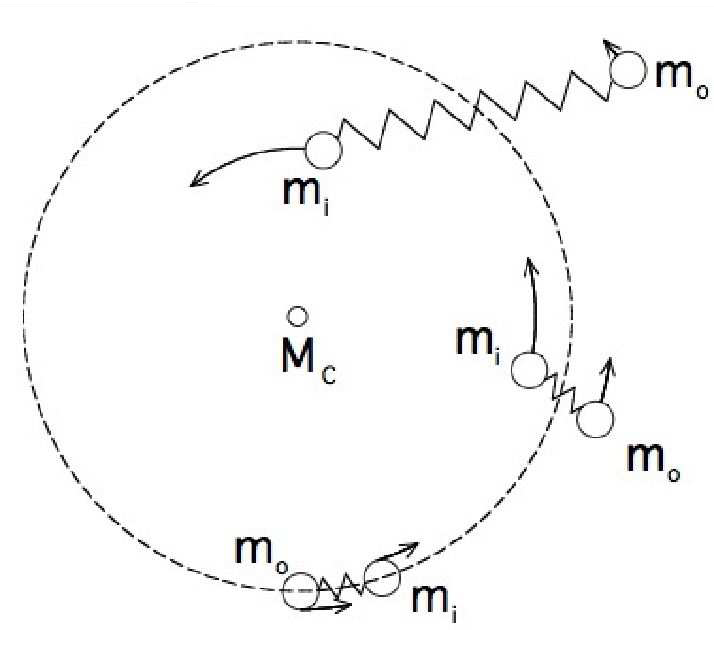
\includegraphics[width=0.35\textwidth]{Balbus2009_diagram}
        \caption{A schematic diagram from \cite{Balbus2009} showing magnetorotational instability. Two fluid elements $m_i$ (inner) and $m_o$ (outer) orbit a mass ($M_C$) with the magnetic tension between the two elements represented by a spring. Over time $m_i$ loses angular momentum, moving closer to $M_C$ while $m_o$ gains angular momentum and moves away from $M_C$.}
        \label{fig:mri}
\end{figure}

One can show that the dispersion relation for the incompressible ideal flow rotating with angular velocity $\Omega_0$ is
\begin{align}
    \omega^4-\left[2\left(k^2 V_A^2\right) +\kappa^2\right]\omega^2 +\left(k^2 V_A^2\right)\left[\left(k^2 V_A^2\right)+r\frac{d \Omega^2}{dr}\right]=0,
\end{align}
where $\omega$ and $k$ are angular frequency and wave number of a perturbation $\xi \propto e^{i(k z+\omega t)}$. $V_A=\frac{B}{\sqrt{\mu \rho}}$ is Alfv\'en speed for the imposed magnetic field $B$. $\kappa^2$ is known as epicylic frequency $\left(\kappa^2=4\Omega_0^2 + r \frac{d \Omega^2}{dr}\right)$ \citep[see][]{Balbus1991,Balbus1998,Balbus2003}. If $\frac{d \Omega^2}{dr}<0$, then one of $\omega^2$ has negative root for long wave length modes satisfying
\begin{align}
    k^2 < -\frac{r}{V_A^2}\frac{d\Omega^2}{dr}.
\end{align}

Therefore, the instability criterion for the magnetorotational instability (MRI) is represented as radially decreasing angular velocity,
\begin{align}
    \frac{d \Omega^2}{dr}<0 \quad \text{(UNSTABLE)}
\end{align} 

Note that the MRI is different from the conventional hydrodynamic instability known as Couette-Taylor centrifugal instability \cite[see][]{Charru2011}. The Couette-Taylor centrifugal instability criterion for axsymmetric perturbation is represented as radially decreasing angular momentum,
\begin{align}
    \frac{d r^4 \Omega^2}{dr} <0 \quad \text{(UNSTABLE)}
\end{align}

The Keplerian disk is a good example of flows which are stable to the hydrodynamic instability but unstable to the MRI.



%--------------------------------------------------
% THEORY
%--------------------------------------------------
\section{Theoretical Work}
\label{sec:theory}

\cite{Acheson1973} and \cite{Knobloch1992} showed the linear stability analysis
of rotating magneto-fluid bounded in coaxial cylinder. For the case of gaseous 
astrophysical disks in unbounded geometry was shown in \cite{Balbus1991}. The 
condition for stability was shown to be radially increasing angular velocity 
profile. We present a linear stability analysis of MRI for radially bounded case 
following \cite{Acheson1972}, \cite{Acheson1973a}, \cite{Knobloch1992}, and 
\cite{Julien2010}.


%
% GOVERNING EQUATIONS
%
\subsection{Governing equation}

The wave dispersion equation of a cylindrical magneto-fluid can be obtained 
from the magnetohydrodynamic (MHD) equations. Assuming the fluid is inviscid 
and perfectly conducting, the ideal MHD equations are 
\begin{align}
    \rho\left(\frac{\partial\mathbf{u}}{\partial t}+\mathbf{u}\cdot\del\mathbf{u}\right) &= -\del p +\mathbf{J}\times\mathbf{B} \\
    \frac{\partial \rho}{\partial t} + \del\cdot(\rho \mathbf{u})&=0 \\
    \frac{d}{dt}\left(\frac{p}{\rho^\gamma}\right)&=0\\
    \mathbf{E}+\mathbf{u}\times\mathbf{B}&=0 \\
    \del\times \mathbf{E} &= -\frac{\partial \mathbf{B}}{\partial t} \\
    \del \times \mathbf{B} &= \mu \mathbf{J},
\end{align}
where $\mathbf{u}$ fluid velocity, $\rho$ is fluid denstity, $p$ is pressure. $d/dt=\partial/\partial t +\mathbf{u}\cdot\del$ is convective derivative and $\gamma$ is the ratio of specific heats. $\mathbf{E}$, $\mathbf{B}$ and $\mathbf{J}$ are electic field, magnetic field and current density respectively \cite[see][]{Freidberg1987}.

To investigate the magnetorotational instability, one can consider homogeneous incompressible fluid rotating 
with angular velocity $\Omega(r)=\frac{V(r)}{r}$ in externally imposed magnetic 
fields $\mathbf{B}_0 = [0,B_\phi(r),B_z(r)]$. Combining electromagnetic 
equations with momentum relation, we get the appropriate MHD equations,
\begin{align}
    \frac{\partial \mathbf{u}}{\partial t}+(\mathbf{u}\cdot\del)\mathbf{u} &= -\frac{1}{\rho}\del\left(P+\frac{\mathbf{B}^2}{2\mu}\right)+\frac{1}{\mu\rho}(\mathbf{B}\cdot\del)\mathbf{B}\\
    \frac{\partial \mathbf{B}}{\partial t} +(\mathbf{u}\cdot\del)\mathbf{B} &=(\mathbf{B}\cdot\del)\mathbf{u} \\
    \del\cdot\mathbf{u}&=0\\
    \del \cdot \mathbf{B} &=0.
\end{align}


%
% LINEARIZATION
%
\subsection{Linear perturbation equation and eigenvalue problem}

We can get linearized equations by perturbing the basic state by small amount
of $\mathbf{u_1}$ and $\mathbf{b_1}$ for velocity and magnetic fields.
%\begin{align}
%\frac{\partial \mathbf{u}_1}{\partial t} +(\mathbf{u}_0\cdot \del)\mathbf{u}_1 &= -\frac{1}{\rho}\del\left(p_1+\frac{\mathbf{B}_0\cdot\mathbf{B}_1}{\mu}\right) +\frac{\mathbf{B}_0\cdot\del\mathbf{B}_1+\mathbf{B}_1\cdot\del\mathbf{B}_0}{\mu \rho}-(\mathbf{u}_1\cdot \del)\mathbf{u}_0\\
%\frac{\partial \mathbf{B}_1}{\partial t}+(\mathbf{u}_0\cdot \del)\mathbf{B}_1 &= (\mathbf{B}_0\cdot \del)\mathbf{u}_1+(\mathbf{B}_1\cdot \del)\mathbf{u}_0-(\mathbf{u}_1\cdot \del)\mathbf{B}_0\\
%\del\cdot \mathbf{u}_1&=0\\
%\del \cdot \mathbf{B}_1 &=0
%\end{align}
The linear perturbation is assumed to have the form
\begin{align}
    f=\Re\left[\hat{f}(r)e^{i(m\phi+kz+\omega t)} \right].
\end{align}
Accoring to \cite{Acheson1972}, the normal mode equations are
\begin{align}
\hat{b}_r &=\frac{\hat{u}_r}{\omega}\left(k B_z +\frac{m B_\phi}{r}\right),\\
\hat{b}_\phi &= -\frac{(\hat{u}_r B_\phi)'}{i\omega} +\frac{k}{\omega}(\hat{u}_\phi B_z -\hat{u_z}B_\phi),\\
\hat{b}_z &= -\frac{(r\hat{u}_r B_z)'}{ri\omega} - \frac{m(\hat{u_\phi} B_z - \hat{u}_z B_\phi)}{r\omega},\\
\hat{u}_z &= -\frac{(r\hat{u}_r)'}{rik}-\frac{m\hat{u}_\phi}{rk},\\
\left(1+\frac{m^2}{r^2k^2}\right)ri\hat{u}_\phi &= -\frac{m}{rk^2}(r\hat{u}_r)' \nonumber \\ &-\frac{\hat{u}_r}{\left(V_{Az}+\frac{m V_{A\phi}}{rk}\right)^2\frac{k^2}{\omega^2}-1}
\left\{-\frac{2\Omega r}{\omega}+\frac{2kV_{A\phi}}{\omega^2}\left(V_{Az}+\frac{mV_{A\phi}}{rk}\right)\right\},
\end{align}
%\begin{align}
%    -i\omega\hat{b}_r&= ikB_z \hat{u}_r\\
%    -i\omega\hat{b}_\phi &= -\frac{d}{dr}(\hat{u}_r B_\phi) +ik(\hat{u}_\phi B_z -\hat{u}_z B_\phi)\\
%    -i\omega \hat{b}_z &= -\frac{1}{r}\frac{d}{dr} (r\hat{u}_r B_z)\\
%    ik\hat{u}_z &= -\frac{1}{r}\frac{d}{dr}(r \hat{u}_r)\\
%    i{(\omega^2-k^2 V_{Az}^2)}\hat{u}_\phi &= %\frac{\hat{u}_r}{r}(2\Omega r \omega +2k V_{A\phi}V_{Az})
%\end{align}
where $V_{A\phi}=\frac{B_\phi (r)}{\sqrt{\mu\rho}}$, $V_{Az}=\frac{B_z (r)}{\sqrt{\mu\rho}}$ are Alfv\'en speeds for associated external magnetic field components.

Solving the normal mode equation set for radial velocity perturbation 
$\hat{u}_r = u$ and considering axisymmetric perturbation $(m=0)$, \cite{Acheson1973a} obtained following eigenvalue problem,
\begin{align}
    \frac{d}{dr}\left[(\omega^2-k^2 V_{Az}^2)\left(\frac{du}{dr}+\frac{u}{r}\right)\right]-k^2\left[\omega^2-k^2 V_{Az}^2+r\frac{d}{dr}\left(\frac{V_{A\phi}^2}{r^2}-\frac{V^2}{r^2}\right)\right]u \nonumber \\
    = -\frac{4 k^2}{r^2}\frac{(k V_{A\phi} V_{Az}+\omega V)^2}{(\omega^2-k^2 V_{Az}^2)} u.
\end{align}


%
% STABILITY
%
\subsection{Stability criterion}

\subsubsection{Standard magnetorotational instability}

Consider a standard MRI of radially bounded coaxial fluid cylinder with 
externally imposed axial magnetic field but without axial current flowing. 
Therefore, we have $V_{Az}=\frac{B_z}{\sqrt{\rho\mu}}=const \neq 0$ and 
$V_{A\phi}=\frac{B_\phi}{\sqrt{\rho\mu}}=0$. Considering boundary condition 
$u(r_1)=u(r_2)=0$, we multiply the eigenvalue equation by complex conjugate 
of $u$ and integrate over radial coordinate,
\begin{align}
    (\omega^2-k^2 V_{Az}^2)^2 = \frac{k^2}{D}\int_{r_1}^{r_2}\left[\frac{\omega^2}{r^2}\frac{d}{dr}r^2V^2 -r^2 k^2 V_{Az}^2 \frac{d}{dr}\left(\frac{V^2}{r^2}\right)\right]|u|^2 dr
\end{align}   
where 
\begin{align}
    D\equiv \int_{r_1}^{r_2}\left(r \left|\frac{du}{dr}\right|^2 +\frac{|u|^2}{r}+k^2 r |u|^2 \right) dr >0
\end{align}

Accoring to \cite{Chandrasekhar1960}, $\omega^2$ must be real. We get stable 
modes with $\omega^2>0$ and unstable modes with $\omega^2<0$. If the angular 
velocity increases radially outward, $\frac{d}{dr}\left(\frac{V^2}{r^2}\right)>0$, 
the system is stable because $\omega^2$ is bounded from below by positive number, 
\begin{align}
    \omega^2>\frac{r^2k^2 V_{Az}^2 \frac{d}{dr}\left(\frac{V^2}{r^2}\right)}{4\frac{V^2}{r}+r^2\frac{d}{dr}\left(\frac{V^2}{r^2}\right)}>0.
\end{align}
If we have radially decreasing anguar velocity profile, 
$\frac{d}{dr}\left(\frac{V^2}{r^2}\right)<0$, somewhere $r_1<r<r_2$, then 
$\omega^2$ may have negative solution which makes the system unstable.

\subsubsection{Helical magnetorotational instability}

When the external nonzero magnetic fields in axial and azimuthal directions are
considered, it was found that the eigenvalue equation can be written as
\begin{align}
    \frac{d}{dr}r\frac{du}{dr}-\frac{u}{r}-k^2ru = \frac{k^2}{(\omega^2-k^2 V_{Az}^2)^2}\left[r^2 \frac{d}{dr}\left(\frac{V_{A\phi}^2-V^2}{r^2}\right)
    (\omega^2-k^2V_{Az}^2) 
    -\frac{4}{r}(kV_{A\phi}V_{Az}-\omega V)^2\right]u
\end{align}

According to \cite{Knobloch1992} and \cite{Julien2010}, the exponentially 
growing mode $\omega =-i\lambda$, $\lambda>0$ is possilbe when the eigenvalue 
relation has following form
\begin{align}
    (\lambda^2 +k^2 V_{Az}^2)^2 = \frac{k^2}{D}\int_{r_1}^{r_2} \left[ r^2 \frac{d}{dr}\left( \frac{V_{A\phi}^2-V^2}{r^2}\right)(\lambda^2+k^2 V_{Az}^2) + \frac{4}{r}(k V_{A\phi} V_{Az}-i\lambda V)^2 \right]|u|^2 dr.
\end{align}

Considering the imaginary part of the equation, we have 
\begin{align}
    \int_{r_1}^{r_2} \frac{1}{r}V_\phi V |u|^2 dr =0
\end{align}

\cite{Knobloch1992} showed that exponentially growing instability is only possible 
when $V_{A\phi}$ or $V$ changes sign somewhere in $r_1< r < r_2$.


%--------------------------------------------------
% EXPERIMENTS
%--------------------------------------------------
\section{Laboratory Experiments}
\label{sec:experiments}

Experiments: Donnelly and Ozima 1960 = use magnetic fields to stabilize 
centrifugal instability of Taylor-Couette flow; Ji et al. 2001 and others = 
use magnetic fields to generate instability in otherwise stable Taylor-Couette flow

Three types of MRI experiments: 1) standard MRI = axial magnetic field, 2) 
helical MRI = axial and azimuthal magnetic fields, 3) azimuthal MRI = only 
azimuthal magnetic fields

%
% STANDARD
%
\subsection{Standard MRI}
Axial magnetic field

\cite{Ji2001}, \cite{Ji2002} = first modern MRI experiments

\cite{Sisan2004} = inner rotating (copper) sphere, outer fixed (steel) sphere, 
liquid sodium; found $\beta_c$ above which MRI occurred.

\begin{figure}[t]
    \centering
    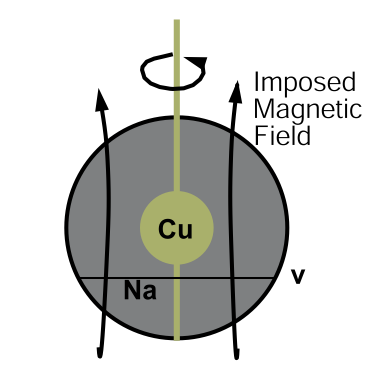
\includegraphics[width=0.35\textwidth]{Sisan2004_diagram}
    \caption{Diagram from \cite{Sisan2004} showing the experimental setup. The fixed outer steel sphere contains liquid sodium (the conducting fluid), with the magnetic field imposed coaxially to the rotating inner copper sphere. The magnetic fields and fluid velocity are measured using Hall probes and Doppler velocimetry.}
\end{figure}


Obstacles of standard MRI in lab experiments: keeping background flow laminar 
(to ensure that the first instability was MRI and not turbulence); minimize 
Ekman effect; achieve high enough speeds without breaking experiment


%
% HELICAL MRI
%
\subsection{Helical MRI}

\cite{Hollerbach2005} = proposed helical (axial + azimuthal magnetic fields) 
to allow MRI at lower Reynolds

\cite{Stefani2006, Stefani2007}  = experimentally proved helical MRI

\cite{Stefani2009} = improve helical MRI experiment


%
% AZIMUTHAL
%
\subsection{Azimuthal MRI}
Azimuthal magnetic fields only (no axial)



%--------------------------------------------------
% NUMERICAL WORK
%--------------------------------------------------
\section{Numerical Work}

MRI: occurs in a Rayleigh-Stable regime whenever a weak poloidal magnetic 
field is present.

Accretion can only occur with a efficient mechanism for outward transport of 
angular momentum. There are many suggested processes that can lead to efficient
accretion but none leads to substantial outward angular momentum transport. 
Before using any model, there is a need to understand the angular momentum 
transport characteristics so that the appropriate equations can be used. The 
flow could be turbulent but there is no clear reason why there would be 
turbulence since there is no known instability that will encourage turbulent 
flow.

Numerical simulations are employed to try to explain the anomalous viscosity 
and magnetic field generation. Viscous stresses is insufficient for explaining 
the outward transport of angular momentum so there is a need for some other 
mechanism. Purely hydrodynamic flow will not generate that as will be shown by
HGB and a weak magnetic field is needed. A strong magnetic field will suppress
MRI as shown by \cite{Liu2008}. From linear stability analysis of the exact 
nonlinear streaming solution done by \cite{Goodman1994}, we know the magnetic
field perturbations grows exponentially, indicating that the solution is 
unstable. 3D numerical simulation will help to confirm this analysis.

Direct numerical simulations (DNS) are done to solve the magnetohydrodynamic 
equations for: compressible and incompressible; ideal and non-ideal; 2D and 3D;
axisymmetric and non-axisymmetric; field strength; resolution; computational 
domain size; incorporation of coriolis; and tidal forcing.

With regards to 2D vs 3D simulations, a good comparison was done by 
\cite{Hawley1995} HGB where they did a local shearing box model which 
incorporated coriolis and tidal forcing but neglects background gradients in 
pressure and density (not important unless radial oscillations are 
significant). Periodic boundary conditions were used with an added shearing 
component to the radial direction. " Method of characteristics-constrained 
transport" algorithm as explained in \cite{Hawley1995} was implemented.

The comparison of the 3D simulations results from HGB with the 2D results 
from Balbus et al BGH 1994 shows significant difference. The 2D results have
a general channel/streaming flow solution whereas the 3D results may go through
the channel flow but eventually evolves further into a turbulent flow with some
not going through the channel flow at all. Note: vertical component of gravity,
hence buoyancy, was  ignored and since their simulations showed significant 
density contrast, the shearing box model is not self-consistent. Purely 
hydrodynamic turbulence did not give significant angular momentum transport 
needed even when the initial conditions had strong turbulence structures. 
Their 3D results suggest that accretion disks are well described by Euler's, 
ignoring the viscous terms from Navier Stokes.

Squire's theorem says that for each unstable 3D disturbances, there are 
corresponding 2D disturbance that are more unstable. How does that apply here?

Non-axisymmetric \cite{Fleming2000} - suggest saturation does occur even when 
Elsasser numb $\Delta \ge 1$ if non-axisymmetric disturbances are allowed to 
evolve.

If Alfven speed is slower than sound speed, equations can be simplified to be 
incompressible since it is not fundamental to the instability \cite{Balbus1991} ...

Incompressible shearing box : \cite{Lesur2007}

\cite{Liu2008} (also Princeton MRI experiments) simulated nonlinear development
of MRI in a non-ideal magnetohydrodynamic Taylor-Couette flow (mimicking an 
on-going experiment) using ZEUS-MP 2.0 code (\cite{Hayes2006}), which is a 
time-explicit, compressible, astrophysical ideal MHD parallel 3D code with 
added viscosity and resistivity for axisymmetric flows in cylindrical 
coordinates. He shows that the saturation of MRI causes a inflowing 'jet' 
feature which is opposite to the usual Ekman circulation and enhances angular
momentum transport radially outward, which is what is needed, agreeing with 
HGB. Note: Stable MRI regime ($ Re \le 1600$) enhances vertical angular 
momentum transport while in unstable MRI regime ($Re \ge 3200$), MRI kicks in, 
resulting in more radial angular momentum transport as compared with vertical.

The use of the shearing box model has its limitations as pointed out by HGB as
they do not permit any dynamics involving the background shear, which is taken
as imposed and constant in space and time. \cite{Regev2008}.. With regards to 
resolution which is tied in with the model used, the efficiency of angular 
momentum transport appears to decrease with improved resolution as shown by 
\cite{Fomang2007}, suggesting that transport rates estimated on basis of ideal
MHD are affected by grid-scale dissipation and overestimate the efficiency of 
angular momentum extraction by MRI. \cite{Kapyla2008} also worked on resolution
dependence of $\alpha$, the Shakura-Sunyaev number and the possible decline of
the angular momentum transport rate with decreasing Pm.

Sawai et al 2013 \cite{Sawai2013} simulated a global 3D MRI axisymmetric, ideal
model. They did not find any channel flow solutions as HGB did. Increasing 
spatial resolution contributed to approximate convergence in the exponential 
growth rate but not that of the saturation of magnetic field due to large 
numerical diffusion.

\cite{Kirillov2012} presents a unifying description of the helical and 
azimuthal versions of MRI, and they also identify the universal character of
the 'Liu' limit $2(1 - 2) \approx - 0.8284$ for the critical Rossby number. 
(From this universal characteristics, they are led to the prediction that the
instability will be governed by a mode with an azimuthal wavenumber that is 
proportional to the ratio of axial to azimuthal applied magnetic field, when
this ratio becomes large and the Rossby number is close to the Liu limit)

\cite{Miller1999} worked on vertically stratified disks using a shearing box
model and found that turbulent magnetised disk can produce a magnetised corona
in laminar flow through MRI.

The influence of viscosity and electrical resistivity on the MRI 
\citep[see][]{Pessah2008}
  
From \cite{Julien2010}: Reduced equations- Case A ($ \delta = \epsilon, \Lambda = O(1) $ )\\*
 a) Single Mode theory \\*
 b) Stress-free boundary conditions \\*
 c) Random initial conditions \\*
 
 Reduced equations- Case B ($  \epsilon =O( \delta), \Lambda \gg 1 $ ) \\*
 a) Single Mode Solutions \\*
 b) Multi-mode Sollutions \\*
 c) Random initial Perturbations \\*
 d) Dissipation and Saturation \\*
 
Note: Accretional ejection instability (AEI), as suggested by \cite{Caunt2011},
gives the same angular momentum transport needed as compared to the global MRI
but the instability requires a fairly strong magnetic field. So need an 
external source, possibly from MRI.



%--------------------------------------------------
% CONCLUSION
%--------------------------------------------------
\section{Conclusion}
Concluding remarks



%--------------------------------------------------
% BIBLIOGRAPHY
%--------------------------------------------------
\bibliographystyle{jfm}
\bibliography{sources}


\end{document}
